% Standalone test file for fig:coupled-loop. Same preamble libraries as
% main.tex so the figure can be ported into §3.3 unchanged once it
% renders cleanly. Compile with: pdflatex _tikz_test_loop
\documentclass[runningheads]{llncs}
\usepackage[utf8]{inputenc}
\usepackage[T1]{fontenc}
\usepackage{amsmath,amssymb,mathtools,bm}
\usepackage{tikz}
\usetikzlibrary{arrows.meta, positioning, calc, fit, backgrounds,
                shapes.geometric, decorations.pathreplacing,
                decorations.pathmorphing, matrix, graphs, quotes}
\usepackage{pgfplots}
\pgfplotsset{compat=1.18}

\begin{document}

\begin{figure}[t]
\centering
\resizebox{\linewidth}{!}{%
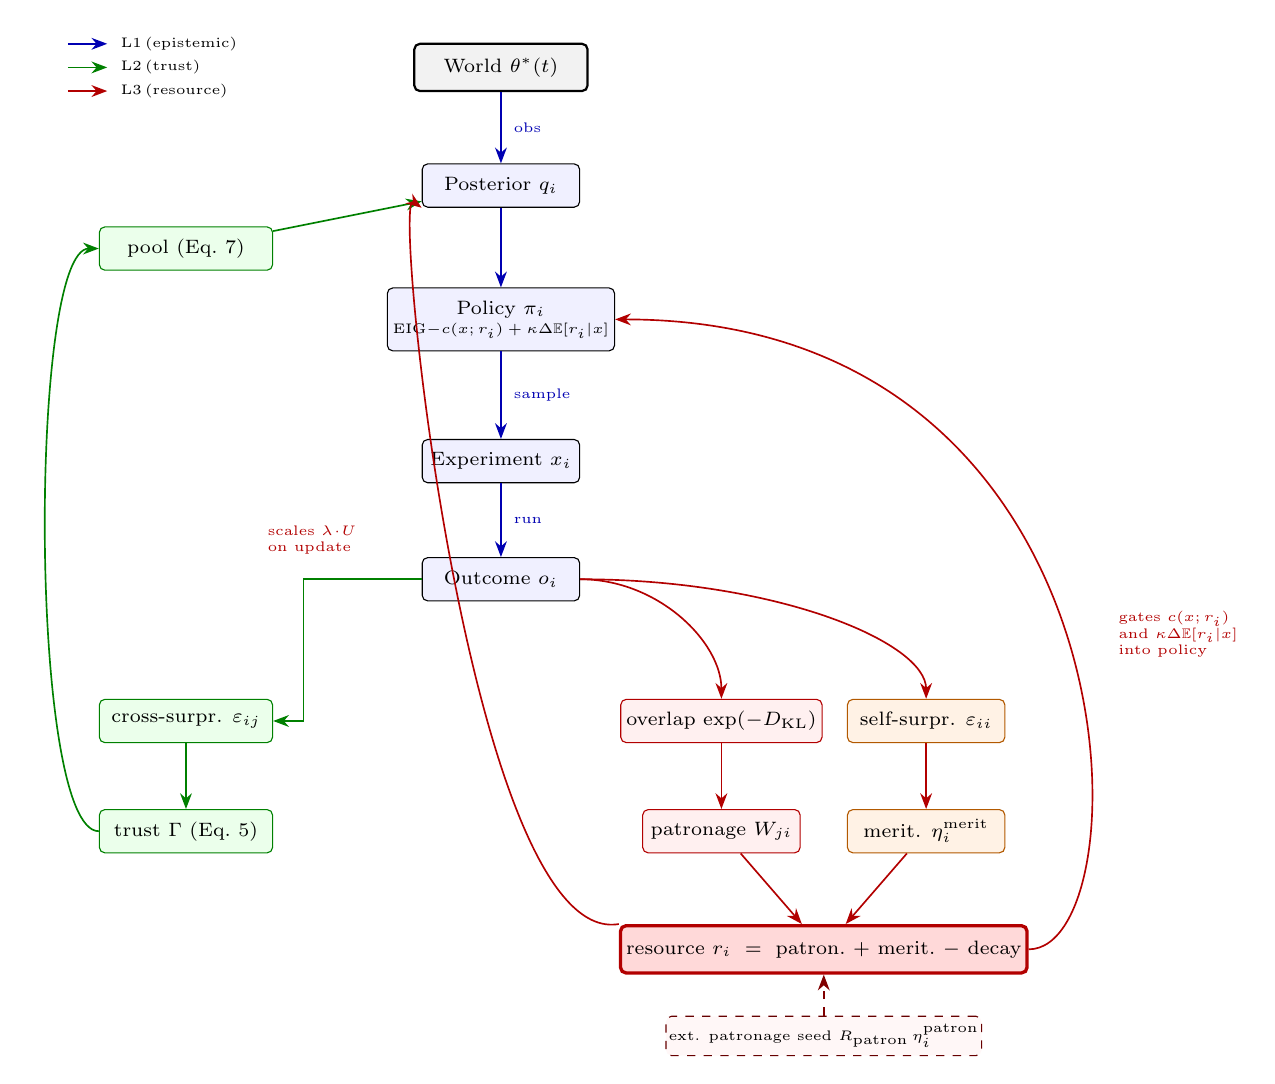
\begin{tikzpicture}[
  >=Stealth,
  font=\scriptsize,
  every node/.style={font=\scriptsize},
  % Node styles
  spine/.style   = {rectangle, draw, rounded corners=2pt,
                    fill=blue!6, minimum width=20mm, minimum height=5.5mm,
                    align=center, inner sep=2pt},
  world/.style   = {rectangle, draw=black, thick, rounded corners=2pt,
                    fill=gray!10, minimum width=22mm, minimum height=6mm,
                    align=center, inner sep=2pt},
  trust/.style   = {rectangle, draw=green!50!black, rounded corners=2pt,
                    fill=green!8, minimum width=22mm, minimum height=5.5mm,
                    align=center, inner sep=2pt},
  patron/.style  = {rectangle, draw=red!70!black, rounded corners=2pt,
                    fill=red!6, minimum width=20mm, minimum height=5.5mm,
                    align=center, inner sep=2pt},
  merit/.style   = {rectangle, draw=orange!70!black, rounded corners=2pt,
                    fill=orange!10, minimum width=20mm, minimum height=5.5mm,
                    align=center, inner sep=2pt},
  rstate/.style  = {rectangle, draw=red!70!black, very thick,
                    rounded corners=2pt, fill=red!15,
                    minimum width=42mm, minimum height=6mm,
                    align=center, inner sep=2pt},
  seed/.style    = {rectangle, draw=red!40!black, dashed, rounded corners=2pt,
                    fill=red!3, minimum width=28mm, minimum height=5mm,
                    align=center, inner sep=1pt, font=\tiny},
  % Arrow styles
  l1/.style      = {->, semithick, blue!70!black},
  l2/.style      = {->, semithick, green!50!black},
  l3/.style      = {->, semithick, red!70!black},
  l3d/.style     = {->, semithick, red!50!black, dashed}
]

% =========================== EPISTEMIC SPINE (L1) ===========================
\node[world]  (W)   at (0,   5.0) {World $\theta^{*}(t)$};
\node[spine]  (Q)   at (0,   3.5) {Posterior $q_i$};
\node[spine, minimum height=8mm]
              (Pi)  at (0,   1.8) {Policy $\pi_i$\\[-1pt]\tiny EIG$-c(x;r_i)+\kappa\Delta\mathbb{E}[r_i|x]$};
\node[spine]  (X)   at (0,   0.0) {Experiment $x_i$};
\node[spine]  (O)   at (0,  -1.5) {Outcome $o_i$};

% L1 vertical arrows
\draw[l1] (W)  -- node[right=1pt, font=\tiny]{obs} (Q);
\draw[l1] (Q)  -- (Pi);
\draw[l1] (Pi) -- node[right=1pt, font=\tiny]{sample} (X);
\draw[l1] (X)  -- node[right=1pt, font=\tiny]{run} (O);

% =========================== TRUST CHANNEL (L2) ===========================
\node[trust]  (Eij)  at (-4.0, -3.3) {cross-surpr. $\varepsilon_{ij}$};
\node[trust]  (Gam)  at (-4.0, -4.7) {trust $\Gamma$ (Eq.~5)};
\node[trust]  (Pool) at (-4.0,  2.7) {pool (Eq.~7)};

\draw[l2] (O.west) -- ++(-1.5,0) |- (Eij);
\draw[l2] (Eij) -- (Gam);
\draw[l2] (Gam.west) .. controls (-6.0, -4.7) and (-6.0, 2.7) .. (Pool.west);
\draw[l2] (Pool) -- (Q);

% =========================== RESOURCE CHANNEL (L3) ===========================
% Two parallel scoring boxes (overlap, self-surprisal)
\node[patron] (Ov)   at (2.8,  -3.3) {overlap $\exp(-D_{\mathrm{KL}})$};
\node[merit]  (Eii)  at (5.4,  -3.3) {self-surpr. $\varepsilon_{ii}$};

% Two update boxes
\node[patron] (Wup)  at (2.8,  -4.7) {patronage $W_{ji}$};
\node[merit]  (Em)   at (5.4,  -4.7) {merit. $\eta^{\mathrm{merit}}_i$};

% Resource state node (centred under the two columns)
\node[rstate] (R)    at (4.1,  -6.2) {resource $r_i$ \;=\; patron.\ + merit.\ $-$ decay};

% External patronage seed - placed below r_i to avoid clash
\node[seed]   (Ps)   at (4.1,  -7.3) {ext. patronage seed $R_{\mathrm{patron}}\,\eta^{\mathrm{patron}}_i$};
\draw[l3d] (Ps) -- (R);

% o_i splits into the two scoring channels with curved paths
\draw[l3] (O.east) .. controls (2.0,-1.5) and (2.8,-2.3) .. (Ov.north);
\draw[l3] (O.east) .. controls (3.5,-1.5) and (5.4,-2.3) .. (Eii.north);

% Scoring → update
\draw[l3] (Ov)  -- (Wup);
\draw[l3] (Eii) -- (Em);

% Updates → r_i
\draw[l3] (Wup) -- (R);
\draw[l3] (Em)  -- (R);

% r_i feeds back: one arrow to Policy (carries c and κΔE), one to Posterior (carries λU)
\draw[l3] (R.east) .. controls (8.2, -6.2) and (8.2, 1.8) .. (Pi.east);
\node[font=\tiny, align=left, red!70!black] at (8.6, -2.2)
  {gates $c(x;r_i)$\\and $\kappa\Delta\mathbb{E}[r_i|x]$\\into policy};
\draw[l3] (R.north west) .. controls (-0.4, -6.2) and (-1.4, 3.5) .. (Q.south west);
\node[font=\tiny, align=left, red!70!black] at (-2.4, -1.0)
  {scales $\lambda\!\cdot\!U$\\on update};

% =========================== LEGEND ===========================
% Inline legend in bottom-left corner, well clear of the trust path
\begin{scope}[shift={(-5.5, 5.0)}, font=\tiny]
  \draw[l1] (0, 0.3)   -- ++(0.5,0); \node[right, font=\tiny] at (0.55, 0.3) {L1\,(epistemic)};
  \draw[l2] (0, 0.0)   -- ++(0.5,0); \node[right, font=\tiny] at (0.55, 0.0) {L2\,(trust)};
  \draw[l3] (0,-0.3)   -- ++(0.5,0); \node[right, font=\tiny] at (0.55,-0.3) {L3\,(resource)};
\end{scope}

\end{tikzpicture}%
}% close resizebox
\caption{The three closed feedback loops of the coupled belief--resource
system, sharing one world--agent--policy--action spine. \textbf{L1
(blue, epistemic)}: standard single-agent active inference, world
$\theta^{*}$ $\to$ posterior $q_i$ $\to$ policy $\pi_i$ $\to$ experiment
$x_i$ $\to$ outcome $o_i$ $\to$ posterior. \textbf{L2 (green, trust)}:
outcomes generate cross-surprisals $\varepsilon_{ij}$ which update the
trust matrix $\Gamma$ (Eq.~5); trust-weighted pooling (Eq.~7) closes the
loop back into $q_i$. \textbf{L3 (red, resource)}: outcomes feed two
parallel scoring channels --- belief overlap drives the patronage flow
$W_{ji}$ (``allocate to those whose beliefs you share''), and
self-surprisal $\varepsilon_{ii}$ drives the meritocratic inflow share
$\eta^{\mathrm{merit}}_i$ (``predictions borne out earn resources'').
Both feed the resource state $r_i$, alongside an external patronage
seed (dashed) controlled by the funding-agency policy. The resource
state then gates two entry points back into the agent's dynamics: a
single arrow into the policy carries both the resource-gated experiment
cost $c(x;r_i)$ and the expected-resource-gain term
$\kappa\Delta\mathbb{E}[r_i|x]$, and a second arrow into the posterior
update scales the $\lambda$-weighted socially-induced utility $U$
pulling $q_i$ toward the beliefs of resource-rich neighbours. \textbf{No
loop closes on its own}; each closes through the others.}
\label{fig:coupled-loop}
\end{figure}

\end{document}
